\documentclass[tikz,border=3mm]{standalone}
\usepackage[utf8]{inputenc}
\usepackage[T1]{fontenc}
\usepackage{amsmath,amssymb}
\usepackage{tikz}
\usetikzlibrary{arrows.meta,calc}

\newcommand{\slashbus}[3]{
    \draw[thick, black!60] ($(#1,#2)+(-0.09,-0.13)$) -- ($(#1,#2)+(0.09,0.13)$);
    \node[font=\tiny\bfseries, text=black!65, above=1pt] at (#1,#2) {#3};
}

\begin{document}
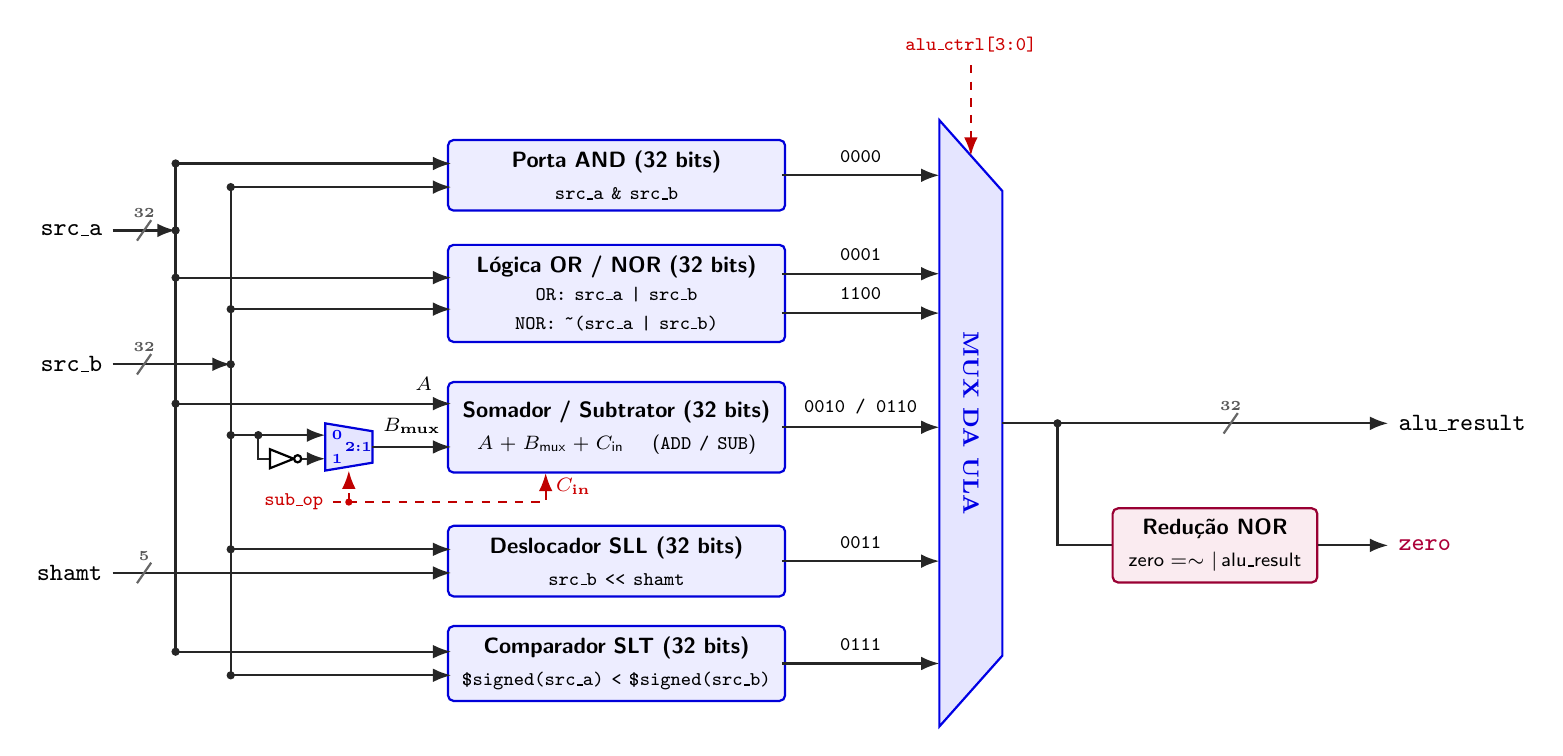
\begin{tikzpicture}[
    >=Latex,
    font=\sffamily\footnotesize,
    funcbox/.style={
        draw=blue!85!black,
        fill=blue!7,
        thick,
        rounded corners=2pt,
        minimum width=4.2cm,
        text width=4.0cm,
        align=center,
        inner sep=4pt
    },
    flagbox/.style={
        draw=purple!80!black,
        fill=purple!8,
        thick,
        rounded corners=2pt,
        align=center,
        inner sep=4pt
    },
    minimux/.style={
        draw=blue!85!black,
        fill=blue!10,
        thick
    },
    muxbox/.style={
        draw=blue!90!black,
        fill=blue!10,
        thick
    },
    bus/.style={->, thick, draw=black!85},
    wire/.style={thick, draw=black!85},
    ctrl/.style={->, dashed, thick, draw=red!75!black},
    ctrlwire/.style={dashed, thick, draw=red!75!black}
]

    % =========================================================================
    % 1. BLOCOS DE OPERAÇÃO DA ULA (Coluna Central, x = 6.4)
    % Largura fixa = 4.2cm -> Bordas: x_west = 4.3, x_east = 8.5
    % =========================================================================
    \node[funcbox] (b_and) at (6.4, 2.9) {
        \textbf{Porta AND (32 bits)}\\[2pt]
        \scriptsize\texttt{src\_a \& src\_b}
    };

    \node[funcbox, minimum height=1.15cm] (b_or) at (6.4, 1.4) {
        \textbf{Lógica OR / NOR (32 bits)}\\[2pt]
        \scriptsize\texttt{OR:  src\_a | src\_b}\\[1pt]
        \scriptsize\texttt{NOR: \textasciitilde(src\_a | src\_b)}
    };

    \node[funcbox, minimum height=1.15cm] (b_adder) at (6.4, -0.3) {
        \textbf{Somador / Subtrator (32 bits)}\\[2pt]
        \scriptsize$A + B_{\text{mux}} + C_{\text{in}}$ \quad (\texttt{ADD / SUB})
    };

    \node[funcbox] (b_sll) at (6.4, -2.0) {
        \textbf{Deslocador SLL (32 bits)}\\[2pt]
        \scriptsize\texttt{src\_b << shamt}
    };

    \node[funcbox] (b_slt) at (6.4, -3.3) {
        \textbf{Comparador SLT (32 bits)}\\[2pt]
        \scriptsize\texttt{\$signed(src\_a) < \$signed(src\_b)}
    };

    % =========================================================================
    % 2. ENTRADAS PRINCIPAIS E BARRAMENTOS DE DISTRIBUIÇÃO (Esquerda)
    % =========================================================================
    % Ponto de entrada das portas principais
    \coordinate (in_a)     at (0.0,  2.2);
    \coordinate (in_b)     at (0.0,  0.5);
    \coordinate (in_shamt) at (0.0, -2.15);

    % Rótulos e fios das entradas
    \draw[bus] (in_a) -- (0.8, 2.2)
        node[at start, left, font=\small\bfseries] {\texttt{src\_a}};
    \slashbus{0.4}{2.2}{32}

    \draw[bus] (in_b) -- (1.5, 0.5)
        node[at start, left, font=\small\bfseries] {\texttt{src\_b}};
    \slashbus{0.4}{0.5}{32}

    \draw[bus] (in_shamt) -- (4.3, -2.15)
        node[at start, left, font=\small\bfseries] {\texttt{shamt}};
    \slashbus{0.4}{-2.15}{5}

    % Barramento vertical de src_a (x = 0.8)
    \draw[wire] (0.8, 3.05) -- (0.8, -3.15);
    \fill[black!85] (0.8, 2.2) circle (1.5pt); % Junção com a entrada

    % Derivações de src_a para os blocos
    \draw[bus] (0.8, 3.05) -- (4.3, 3.05); \fill[black!85] (0.8, 3.05) circle (1.5pt); % AND
    \draw[bus] (0.8, 1.60) -- (4.3, 1.60); \fill[black!85] (0.8, 1.60) circle (1.5pt); % OR
    \draw[bus] (0.8, 0.00) -- (4.3, 0.00)  % Somador (Entrada A)
        node[pos=0.90, above=1pt, font=\scriptsize\bfseries] {$A$};
    \fill[black!85] (0.8, 0.00) circle (1.5pt);
    \draw[bus] (0.8, -3.15) -- (4.3, -3.15); \fill[black!85] (0.8, -3.15) circle (1.5pt); % SLT

    % Barramento vertical de src_b (x = 1.5)
    \draw[wire] (1.5, 2.75) -- (1.5, -3.45);
    \fill[black!85] (1.5, 0.5) circle (1.5pt); % Junção com a entrada

    % Derivações de src_b para os blocos
    \draw[bus] (1.5, 2.75) -- (4.3, 2.75); \fill[black!85] (1.5, 2.75) circle (1.5pt); % AND
    \draw[bus] (1.5, 1.20) -- (4.3, 1.20); \fill[black!85] (1.5, 1.20) circle (1.5pt); % OR
    \draw[bus] (1.5, -1.85) -- (4.3, -1.85); \fill[black!85] (1.5, -1.85) circle (1.5pt); % SLL
    \draw[bus] (1.5, -3.45) -- (4.3, -3.45); \fill[black!85] (1.5, -3.45) circle (1.5pt); % SLT

    % =========================================================================
    % 3. CONDICIONAMENTO DO OPERANDO B (Mini-MUX 2:1 e Inversor NOT)
    % =========================================================================
    % Saída de src_b em direção ao circuito de B
    \draw[wire] (1.5, -0.40) -- (1.85, -0.40);
    \fill[black!85] (1.5, -0.40) circle (1.5pt);

    % Ramo 0: direto para a entrada 0 do MUX
    \draw[bus] (1.85, -0.40) -- (2.7, -0.40);
    \fill[black!85] (1.85, -0.40) circle (1.5pt); % Derivação

    % Ramo 1: deriva para baixo, passa pelo inversor NOT e entra na porta 1
    \draw[wire] (1.85, -0.40) -- (1.85, -0.70) -- (2.00, -0.70);
    % Símbolo do inversor NOT
    \draw[thick, fill=white] (2.00, -0.58) -- (2.30, -0.70) -- (2.00, -0.82) -- cycle;
    \draw[thick, fill=white] (2.35, -0.70) circle (1.3pt);
    \draw[bus] (2.40, -0.70) -- (2.7, -0.70);

    % Trapézio do Mini-MUX 2:1 de B
    \draw[minimux] (2.7, -0.25) -- (3.3, -0.35) -- (3.3, -0.75) -- (2.7, -0.85) -- cycle;
    \node[font=\tiny\bfseries, text=blue!95!black] at (2.85, -0.40) {0};
    \node[font=\tiny\bfseries, text=blue!95!black] at (2.85, -0.70) {1};
    \node[font=\tiny\bfseries, text=blue!85!black] at (3.12, -0.55) {2:1};

    % Saída B_mux para o somador
    \draw[bus] (3.3, -0.55) -- (4.3, -0.55)
        node[midway, above=1pt, font=\scriptsize\bfseries] {$B_{\text{mux}}$};

    % Sinal de controle sub_op e Carry-in (Cin)
    \node[font=\scriptsize\ttfamily\bfseries, text=red!80!black] (subop_lbl) at (2.3, -1.25) {sub\_op};
    % Seleção do Mini-MUX por baixo
    \draw[ctrl] (subop_lbl.east) -- (3.0, -1.25) -- (3.0, -0.85);
    % Propagação para o Carry-In do Somador
    \draw[ctrl] (3.0, -1.25) -- (5.5, -1.25) -- (5.5, -0.88);
    \fill[red!80!black] (3.0, -1.25) circle (1.3pt);
    \node[font=\scriptsize\bfseries, text=red!80!black] at (5.85, -1.05) {$C_{\text{in}}$};

    % =========================================================================
    % 4. MULTIPLEXADOR PRINCIPAL DE SAÍDA (x = 10.5 a 11.3)
    % =========================================================================
    \draw[muxbox] (10.5, 3.6) -- (11.3, 2.7) -- (11.3, -3.2) -- (10.5, -4.1) -- cycle;
    \node[font=\footnotesize\bfseries, text=blue!90!black] at (10.9, -0.25) {\rotatebox{-90}{MUX DA ULA}};

    % Sinal de controle alu_ctrl[3:0] no topo do MUX
    \draw[ctrl] (10.9, 4.3) -- (10.9, 3.15)
        node[at start, above=1pt, font=\scriptsize\ttfamily\bfseries, text=red!80!black] {alu\_ctrl[3:0]};

    % Conexões puramente horizontais dos blocos para o MUX (x = 8.5 a 10.5)
    \draw[bus] (8.5, 2.90) -- (10.5, 2.90)
        node[midway, above=1pt, font=\scriptsize\ttfamily\bfseries] {0000};
    \draw[bus] (8.5, 1.65) -- (10.5, 1.65)
        node[midway, above=1pt, font=\scriptsize\ttfamily\bfseries] {0001};
    \draw[bus] (8.5, 1.15) -- (10.5, 1.15)
        node[midway, above=1pt, font=\scriptsize\ttfamily\bfseries] {1100};
    \draw[bus] (8.5, -0.30) -- (10.5, -0.30)
        node[midway, above=1pt, font=\scriptsize\ttfamily\bfseries] {0010 / 0110};
    \draw[bus] (8.5, -2.00) -- (10.5, -2.00)
        node[midway, above=1pt, font=\scriptsize\ttfamily\bfseries] {0011};
    \draw[bus] (8.5, -3.30) -- (10.5, -3.30)
        node[midway, above=1pt, font=\scriptsize\ttfamily\bfseries] {0111};

    % =========================================================================
    % 5. SAÍDAS DA ULA: alu_result e zero flag (x = 11.3 em diante)
    % =========================================================================
    \coordinate (out_mux) at (11.3, -0.25);

    % Saída principal alu_result
    \draw[bus] (out_mux) -- (16.2, -0.25)
        node[at end, right, font=\small\bfseries] {\texttt{alu\_result}};
    \slashbus{14.2}{-0.25}{32}

    % Derivação para o detector da flag zero
    \fill[black!85] (12.0, -0.25) circle (1.5pt);
    \draw[wire] (12.0, -0.25) -- (12.0, -1.8) -- (12.7, -1.8);

    % Caixa do Redutor NOR (Flag Zero)
    \node[flagbox, minimum width=2.6cm, minimum height=0.9cm] (b_zero) at (14.0, -1.8) {
        \textbf{Redução NOR}\\[2pt]
        \scriptsize$\text{zero} = \sim|\,\text{alu\_result}$
    };

    % Saída da flag zero
    \draw[bus] (b_zero.east) -- (16.2, -1.8)
        node[at end, right, font=\small\bfseries, text=purple!90!black] {\texttt{zero}};

\end{tikzpicture}
\end{document}
